\begin{figure}[ht]
    \centering

    \begin{subfigure}{0.32\textwidth}
        \centering
        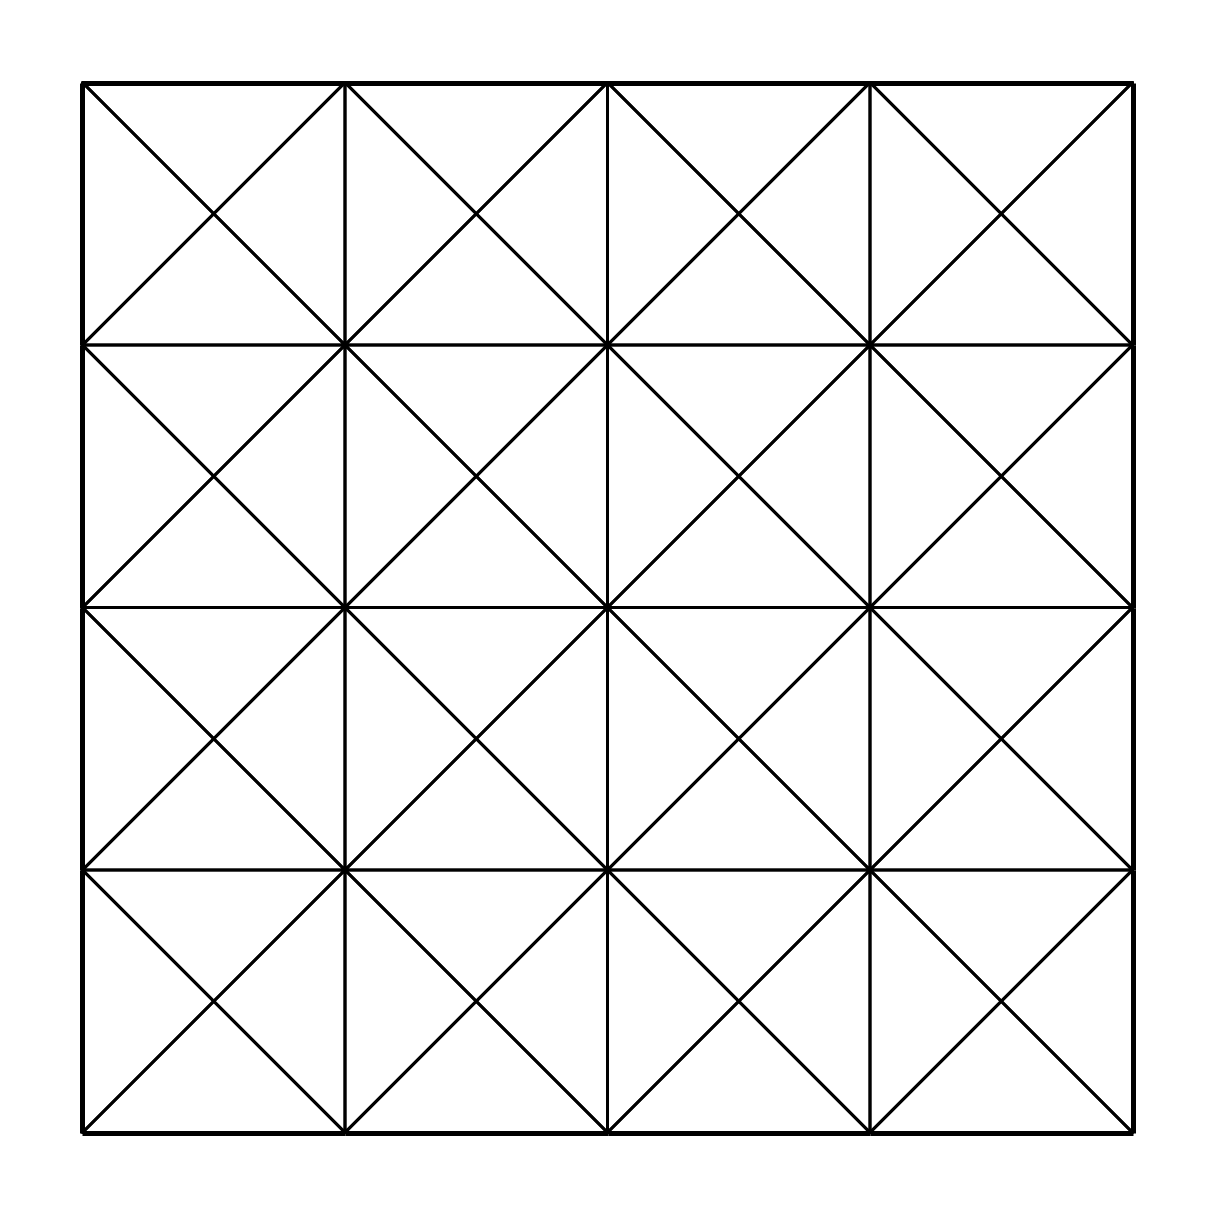
\includegraphics[width=\linewidth]{ThesisDraft/images/crisscross_mesh_N4 (1).png}
        \caption{$N=4$}
    \end{subfigure}
    \hfill
    \begin{subfigure}{0.32\textwidth}
        \centering
        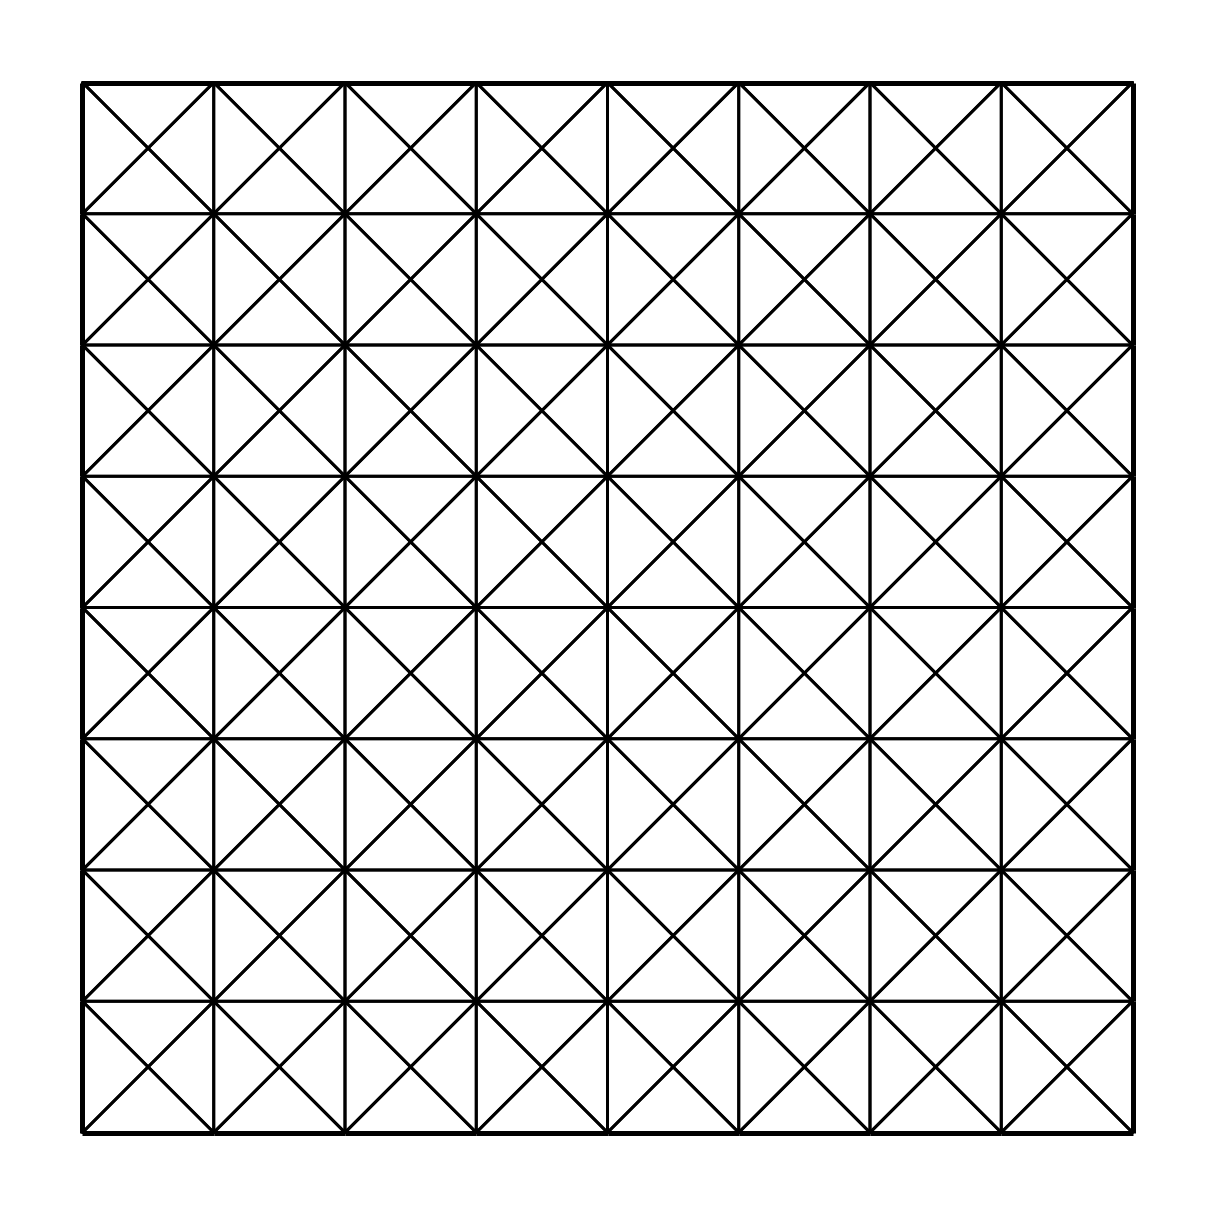
\includegraphics[width=\linewidth]{ThesisDraft/images/crisscross_mesh_N8.png}
        \caption{$N=8$}
    \end{subfigure}
    \hfill
    \begin{subfigure}{0.32\textwidth}
        \centering
        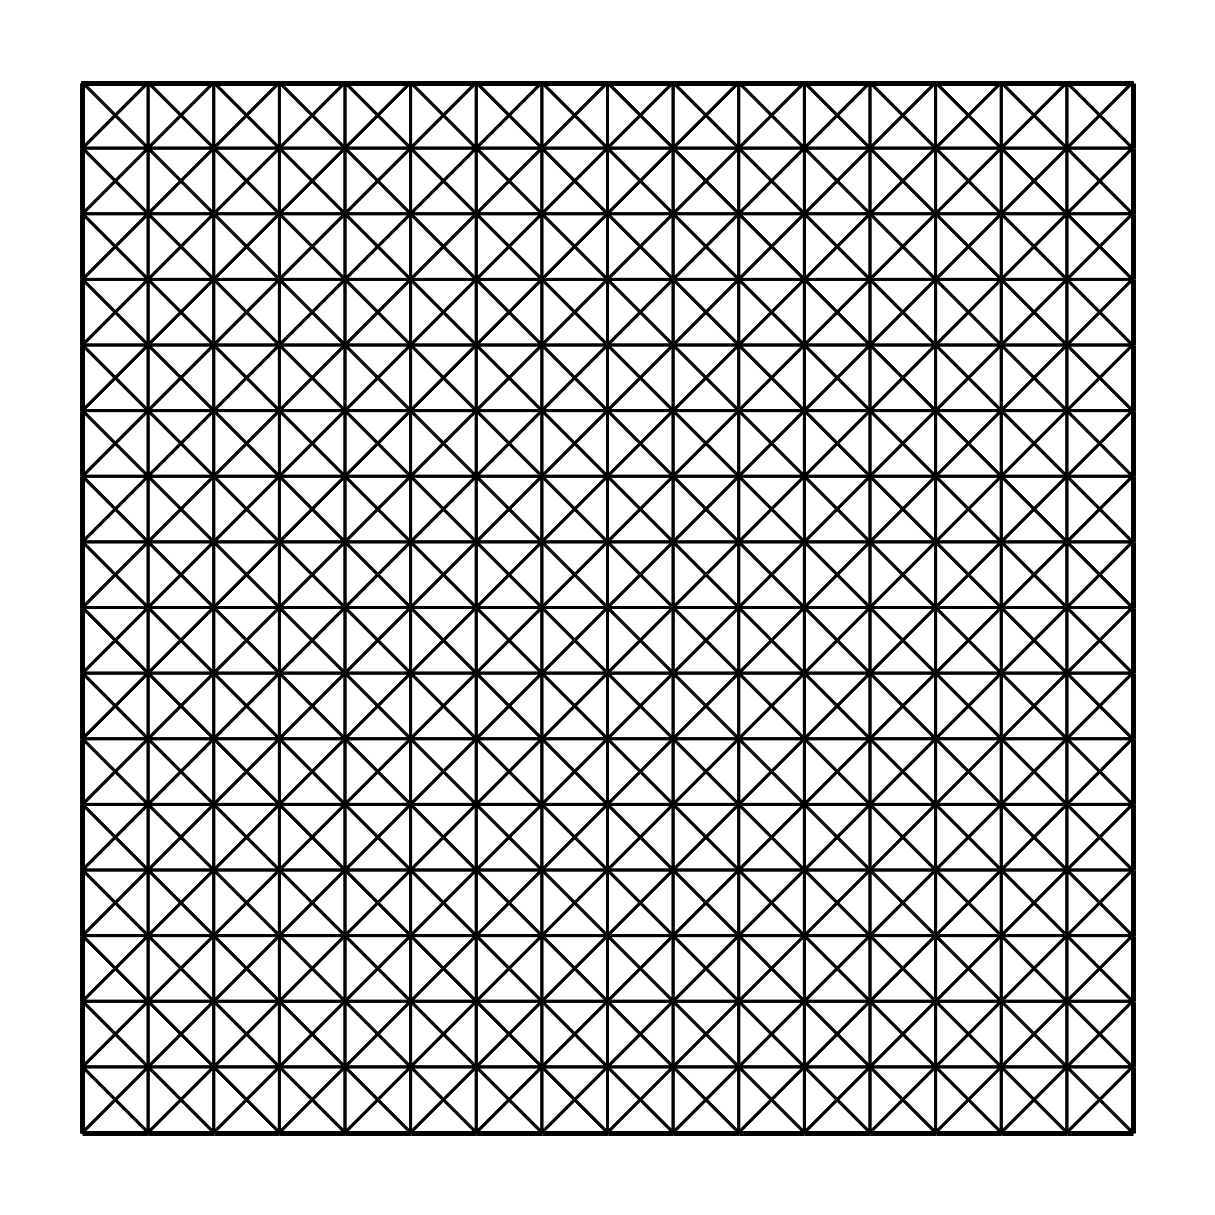
\includegraphics[width=\linewidth]{ThesisDraft/images/crisscross_mesh_N16.png}
        \caption{$N=16$}
    \end{subfigure}

    \caption[Sequence of Criss-Cross Meshes]{The first three meshes in the sequence of criss-cross meshes used to discretize \eqref{2D var max} on $\Omega=(0,\pi)^2$. Here, $N$ denotes the number of cells on each side of the mesh.}
    \label{crisscross}
\end{figure}